%\documentclass[11pt,fleqn]{book}%
%\documentclass{exam}%
\documentclass[11pt,a4paper]{article}
\date{{\LARGE Aprile 2019}}
\usepackage[italian]{babel}
\usepackage[T1]{fontenc}
\usepackage{graphicx}
\usepackage[11pt]{moresize}

\font\myfont=cmr12 at 40pt
\title{{\myfont Sezione d'urto}}

\author{{\Huge Francesco Sacco}\\ \\ \\
		
\includegraphics[scale=0.6]{Immagini/cherubino.eps}\\}
\usepackage[utf8x]{inputenc}
\usepackage{amsmath}
\usepackage{amsthm}
\usepackage{hyperref}

\newcommand{\vettore}[1]{\mathbf{#1}}
\newcommand{\vettorec}[1]{\textrm{#1}}
\newcommand{\pscal}[2]{\langle #1,#2\rangle}

\begin{document}
	\maketitle
	\tableofcontents
	\newpage
	\section*{Prefazione}
		Visto che c'è molta confusione sulla sezione d'urto faccio questi brevi appunti per chiarire bene cos'è e cosa rappresenta.\newline
		Lungo il pdf mettero un bel pò di note a piè di pagina, esse vanno lette solo se non si capisce quello che si sta leggendo, se stai capendo non leggerle,\footnote{Minchia ma allora non hai capito un cazzo} rovinano il flusso della discussione.\newline 
		La sezione d'urto viene indicata di solito con $\sigma$, Il suo nome richiama alla mente qualcosa che abbia a che vedere un'area su cui sbatte qualcosa. Però la sezione d'urto non è sempre l'area dell'oggetto, ma intende rappresentare una sorta di "area equivalente".\newline
		Ad esempio è ragionevole dire che per la luce l'area effettiva di un vetro $1m\times 1m$ è minore di un metro quadro, questo perchè molti fotoni passano attraverso il vetro indisturbati.\newline
	\section{Sezione d'urto s'un oggetto opaco}
	\label{sec:opaco}
		Per semplicità iniziano a trattare il concetto di sezione d'urto nel caso di un oggetto opaco,\footnote{Chiaramente le particelle incidenti sono fotoni, ma con un pò di fantasia si può generalizzare il concetto con oggetti incidenti diversi dai fotoni} in questo caso ci aspettiamo che la sezione d'urto sia uguale alla superfice ortogonale al facio.\newline
		Noi in questo caso vogliamo ricavare l'area ortogonale in base a quello che succede al fascio di luce che lo colpisce.\newline

		Supponiamo di mandare un facio di luce con un'area maggiore del bersaglio, e che dietro ci sia uno schermo ortogonale al facio molto grande che raccolga la luce (figura \ref{fig:ombra}), allora possiamo dire che la sezione d'urto è l'area dell'ombra che l'oggetto genera sullo schermo.\newline
		Chiamarente se l'oggetto è una superfice orientata ortogonalmente al facio luminoso, la sua sezione d'urto sarà uguale alla sua area.\newline
		\begin{figure}
			\centering
    		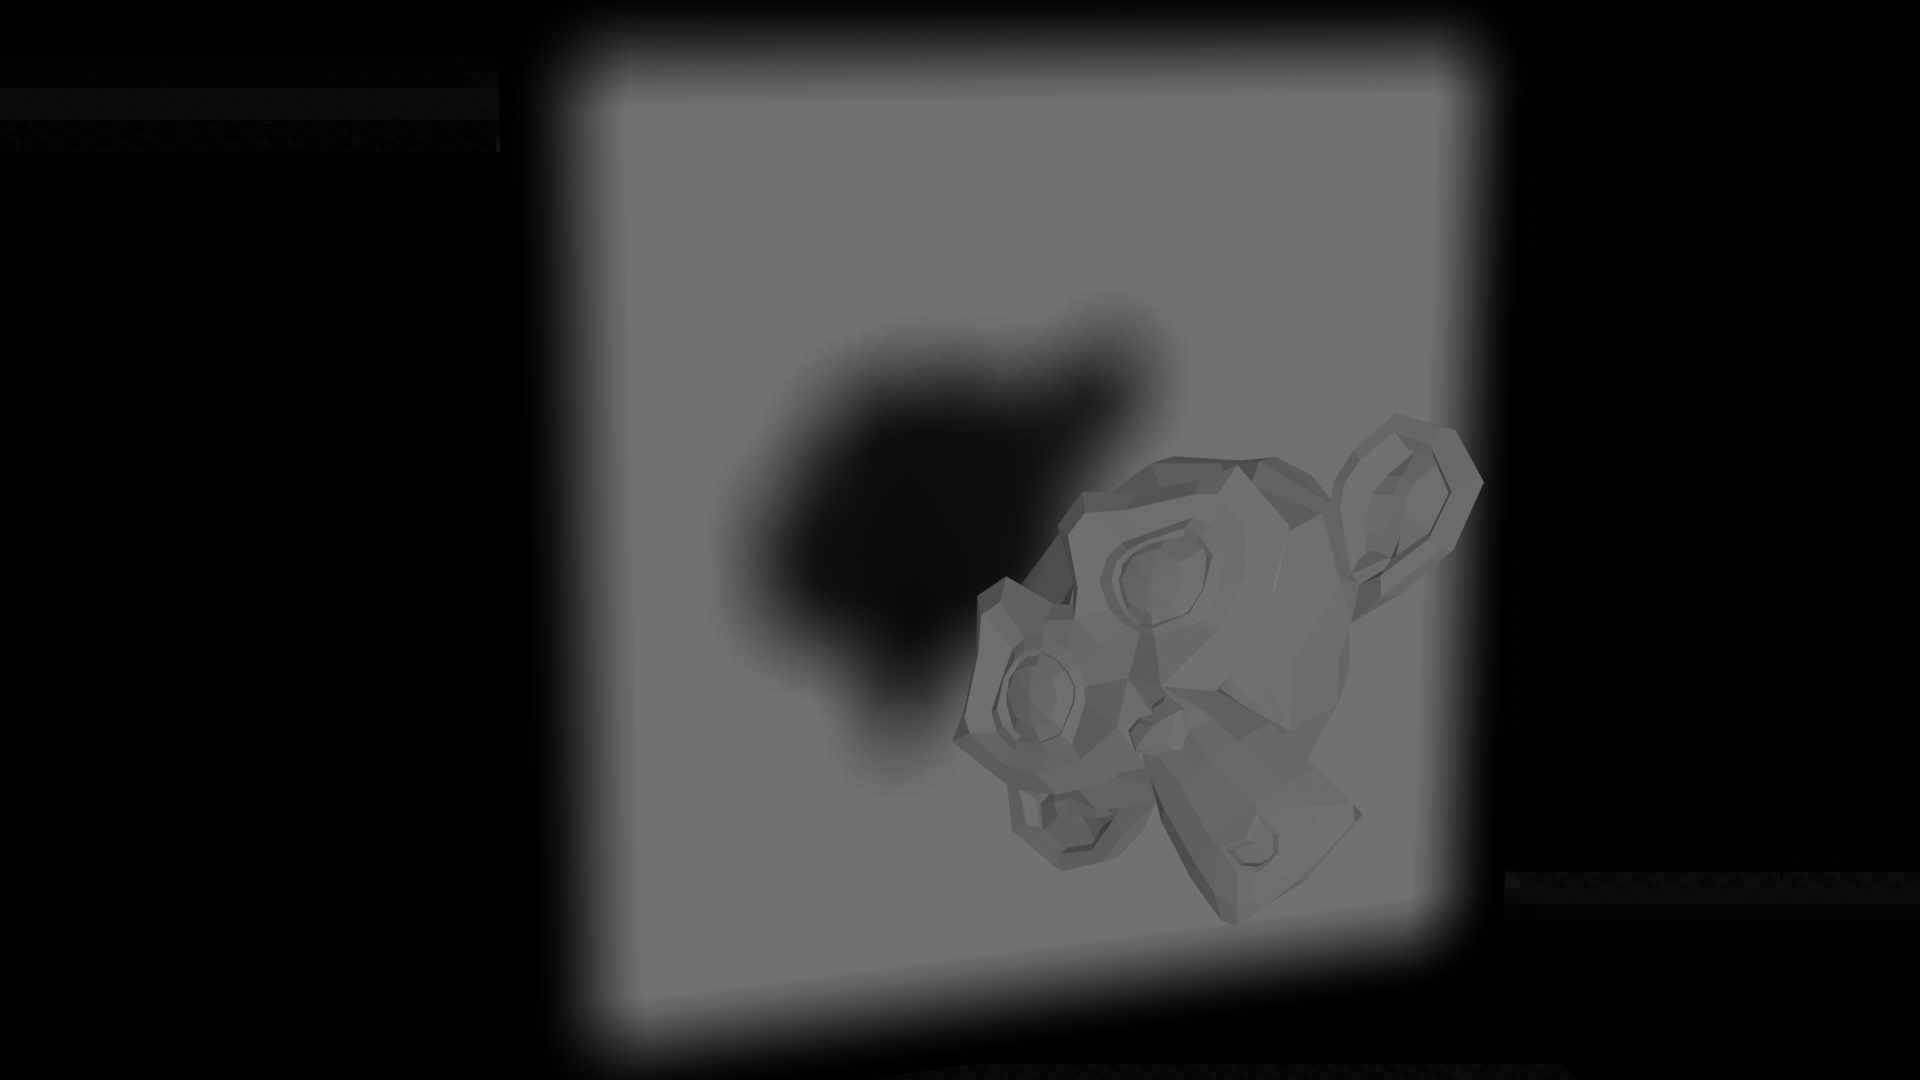
\includegraphics[width=\linewidth]{Immagini/ombra_con_blender.png}
    		\caption{Immagine fatta male illustrativa}
    		\label{fig:ombra}
		\end{figure}

		Solo che c'è un problema: nel caso di un'oggetto sgummato sarà difficile misurare l'area. Per ovviare a questo problema si può mettere uno schermo che sia in grado di contare i fotoni che riceve e una sorgente che sia in grado di contare i fotoni che manda.\newline
		Chiamiamo $A$ l'area illuminata dalla sorgente quando non c'è il bersaglio in mezzo ai piedi, che per comodità la creiamo quadrangolare, $n_s$ il numero di fotoni che colpiscono lo schermo per unità di tempo e $\Phi$ il numero di fotoni che vengono sparati dalla luce per unità di tempo, allora con una semplice proporzione si può dire che:
		\begin{equation}
			\sigma:(n_l-n_s)=A:n_l \rightarrow \sigma=A\cdot(1-n_s/\Phi)
			\label{eq:sigma_luce}
		\end{equation}
		Adesso vediamo se funziona veramente questo ragionamento.\newline
		Per verificare prendiamo un bersaglio quadrato di area $\sigma=1$ illuminata da una luce quadrata di area $A=2$, di conseguenza metà dei fotoni verrà bloccata, cioè $n_s=\Phi/2$, quindi $1=2\cdot(1-\Phi/2\cdot 1/\Phi)=2\cdot(1-1/2)=2\cdot 1/2=1$.\newline
		Che bello funziona.\newline

		Una cosa molto importante che poi verrà applicata è l'additività della sezione d'urto, infatti se prendiamo due schermi opachi quadrati con $\sigma=1$ e li mettiamo uno accanto all'altro formando un rettangolo, esso avrà una sezione d'urto uguale a $2$.

	\section{Sezione d'urto s'un oggetto traslucido}
		Per gli oggetti traslucidi tratteremo soltanto quelli planari, perchè quelli con geometri tridimenzionali si comportano in modo strano con la luce.\footnote{Facendo qualche assunzione volendo si potrebbe trattare anche oggetti tridimenzionali, ma non credo aiuti alla comprenzione del testo}\newline

		Se ti dico:"Io ho una lastra di vetro di un metro quadro che fa passare la metà della luce, qual'è la sezione d'urto?"\footnote{Supponiamo che la luce che non passi venga assorbita, a dire il vero non è molto importante che fine faccia} tu mi risponderai di sicuro:"mezzo metro quadro", ma come è possibile giustificare questa affermazione?\newline

		Chiaramente deriva dall'equazione \ref{eq:sigma_luce}, ma si perde un pò il concetto che invece era ben chiaro con lo schermo opaco che ci ha portato in primo luogo a ricavare quell'equazione.\newline

		Ora però ti porto un'altro vetro traslucido con le esatte stesse proprietà, e ti chiedo:"qual'è la sezione d'urto di quest'altro vetro?", tu mi dirai:"è lo stesso di prima, quindi per forza sarà mezzo metro quadro", e io ti rispondo:"la tua sezione d'urto è esatta, ma ti sbagli a dire che è lo stesso di prima! Questo è uno schermo opaco che ha tantissimi buchetti microscopici che in totale gli levano metà dell'area"\footnote{Chiaramente è un'esperimento mentale, nella realtà fare una cosa del genere non sarà possibile perchè dovrebbe avere uno spessore nullo e la luce ha anche un comportamento ondulatorio che porterebbe alla diffrazione, ma possiamo supporre che tutto questo non accada in questo esempio}.\newline

		Quindi effettivamente possiamo dire che il vetro è un pò come uno schermo opaco con tanti buchettini, e quindi deve avere la stessa sezione d'urto, e quindi si usa l'equazione \ref{eq:sigma_luce}.\newline

	\section{Collegamento con la probabilità}
		Sempre rimandendo nel caso del vetro traslucido posso fare questa affermazione:Se il fotone viene assorbito, allora vuol dire che ha interagito con un'atomo dell vetro, altrimenti è passato indisturbato.\newline

		Ora vogliamo vedere se è possible legare la probalbilirà di interazione $P$ con la sezione d'urto.\newline
		Sempre usando la notazione della sezione \ref{sec:opaco} e dell'equazione \ref{eq:sigma_luce}, possiamo dire che la probabilità $P$ che il fotone incida sia quanti ne vengono assorbiti dal bersaglio per unità di tempo, che sono tanti quanti a quellli che non arrivano sullo schermo per unità di tempo $N_i=(\Phi-n_s)$, diviso quanto ne arrivano in totale $\Phi$, quindi:
		\begin{equation}
			P=\frac {N_i} \Phi=\Big(1-\frac {n_s}\Phi\Big)=\frac\sigma A
			\label{eq:prob1}
		\end{equation}

	\section{Sezione d'urto di una particella}
		Supponiamo adesso che la luce venga proiettata in modo che ogni singolo fotone colpisca il bersaglio (ma non per forza deve essere assorbito, può anche attraversarlo se è translucito), e che il bersaglio sia un oggetto planare con una densità di atomi per unità di superfice $n_s$.\newline
		Adesso io voglio sapere quantè la sezione d'urto di un atomo sulla superfice, visto che la sezione d'urto è additiva\footnote{come spiegato negli ultimi righi del paragrafo \ref{sec:opaco}} posso dire che la sezione d'urto del bersagio $\sigma_b$ è uguale alla sezione d'urto di un singolo atomo $\sigma$ moltiplicato per quanti ce ne sono per unità di superfice $n_s$ moltiplicato per quanta superfice c'è $A$, quindi:
		\[
			\frac{AN_i}\Phi=\sigma_b=\sigma A n_s
		\]
		dove la prima eguaglianza viene dall'equazione \ref{eq:prob1}, risolvendo per sigma si ottiene che 
		\begin{equation}
			\sigma=\frac{N_i}{\Phi n_s}
		\end{equation}
		Questa equazione però dipende da come è fatta la lastra bersaglio, quindi se vogliamo qualcosa che ne sia indipendente bisogna fare qualche passaggio matematico:
		\[
			\sigma=\frac{N_i}{\Phi n_s}\cdot \frac{An_s}{An_s}=
			\frac{N_i}{An_s}\cdot\frac A\Phi\cdot \frac {n_s}{n_s}=
			N_a\cdot \frac1{|j|}\cdot 1=\frac{N_a}{|j|}
		\]
		Dove ho detto che il numero di interazioni sulla lastra per unità di tempo $N_i$ è uguale al numero di interazioni su un singolo atomo $N_a$ moltiplicato per quanti atomi ci sono $An_s$ (Area per densità), quindi $N_i/(An_s)=N_a$ e poi ho detto che il flusso attraverso l'area $\Phi$ diviso l'area stessa $A$ dà la densità di corrente, quindi $A/\Phi=1/|j|$.\newline
		Mettendo tutti insieme si ha che 
		\begin{equation}
			\sigma=\frac{N_a}{|j|}
		\end{equation}

	\section{Sezione d'urto differenziale}
		Alcune sezioni d'urto per loro natura tendono a divergere. Infatti se consideriamo lo scattering Coulomb tra un flusso di particelle cariche $|j|$ che incide su una carica dello stesso segno si ha che $\sigma=N/|j|=+\infty$ visto che il numero di interazioni al secondo è infinito se consideriamo il flusso incidente come un'infinità di particelle che arrivano al secondo.\newline
		Questo torna al livello intuitivo perchè se la sezione d'urto è l'area all'interno del quale c'è interazione tra proiettile e bersaglio, allora nel caso dell'interazione eletromagnetica deve fare infinito visto che il campo elettrico di una carica si estende all'infinito, anche se più debole.\newline
		Però abbiamo detto che sezione d'urto e probabilità vanno a braccetto, quindi certe volte anzichè chiedersi "Qual'è la probabilità che ...", si ci può chiedere "Qual'è la sezione d'urto tale che ...". Nei puntini chiaramente si ci deve mettere qualcosa che abbia senso nel nostro contesto.\newline
		Adesso ci chiediamo qual'è la sezione d'urto tale che il flusso uscente finisca per andare entro un certo angolo solido infinitesimo $d\Omega$ dopo che avvenga uno scattering coulumbiano, scritto in equazioni sarà così:
		\begin{equation}
			\frac{d\sigma}{d\Omega}=\frac{N(\Omega)}{|j|}
			\label{eq:sez_diff}
		\end{equation}
		$d\sigma$ rappresenta una piccola area, tale che se ci entri poi vai a finire in un angolo solido $d\Omega$, come visibile nell'immagine \ref{fig:rut1} e $N(\Omega)$ è il numero di interazioni al secondo che fanno finire (asintoticamente) i proiettili in un angolo $\Omega$.\newline
		\begin{figure}
			\centering
    		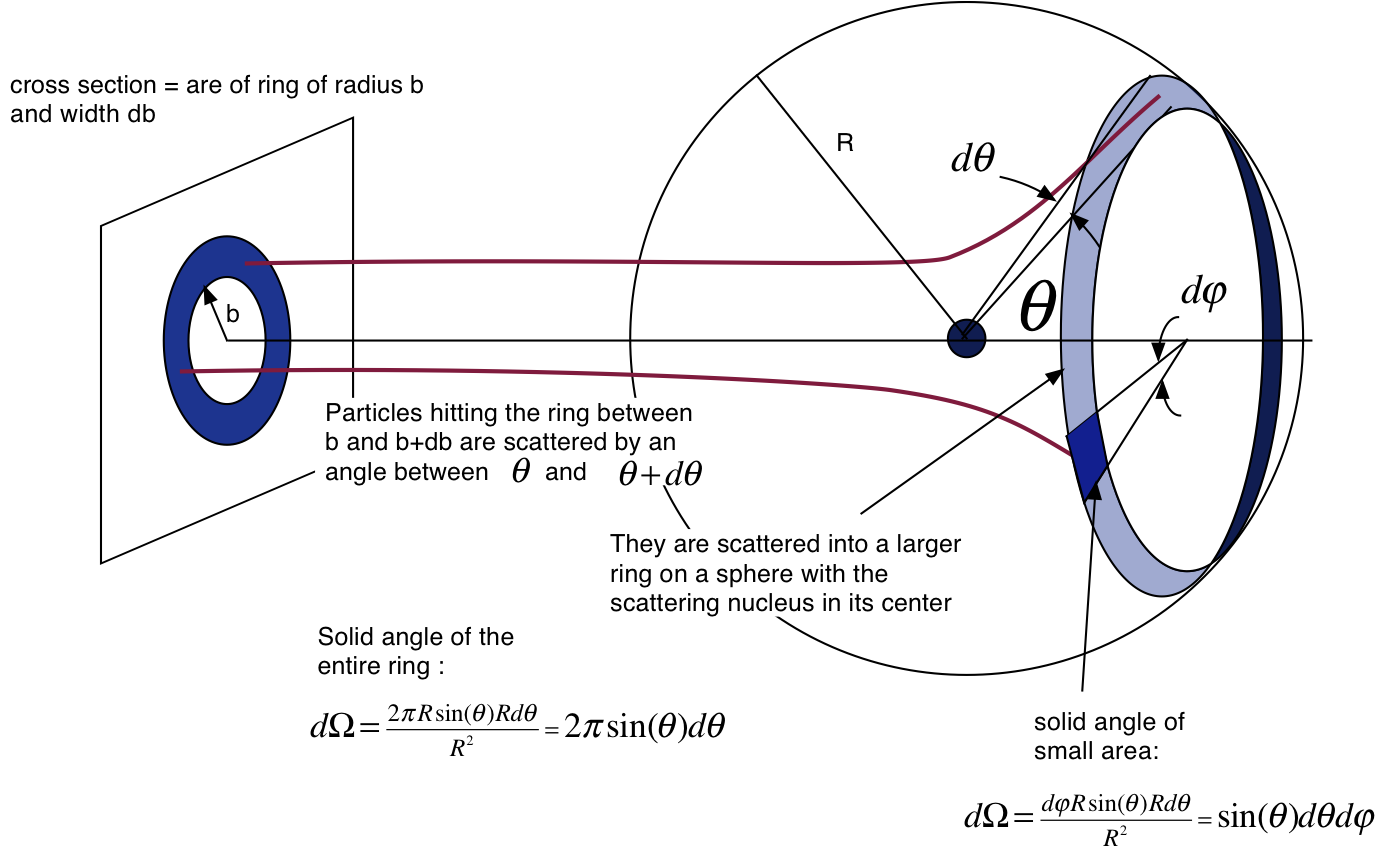
\includegraphics[width=\linewidth]{Immagini/solid_angle.png}
    		\caption{In questo caso $d\sigma=2\pi b db$ e $d\Omega=2\pi \sin(\theta)d\theta$ sono a simmetria cilindrica}
    		\label{fig:rut1}
		\end{figure}
		Questo tipo di scattering è detto "Scattering Rutherford", non mi dedicherò molto a questo argomento perchè è trattato abbastanza bene anche altrove\footnote{Ad esempio nelle dispenze di Claudio Bonati}. Qui dirò soltanto che il risultato finale è che
		\begin{equation}
			\frac{d\sigma}{d\Omega}=\Big(\frac{e_1e_2}{2\mu v_\infty^2 }\Big)\frac{1}{\sin^4(\theta/2)}
		\end{equation}
		dove $\mu$, $e_2$, $v_\infty$ e $\theta$ sono rispettivamente la massa, la carica, la velocità iniziale e l'angolo di deflessione delle particelle cariche proiettile ed $e_1$ è la carica del bersaglio.

	\section{Cose con onde elettromagnetiche}
		Nel caso di onde elettromagnetiche si ci può chiedere:"Una volta che ci siamo calcolati come delle onde elettromangetiche di frequenza $\omega$ vengono diffratte da un'ostacolo, non possiamo calcolarci la sezione d'urto come se fosse stata calcolata con dei fotoni anch'essi di frequenza $\omega$?".\newline
		Effettivamente, se fosse possibile farlo risolverebbe un bel pò di problemi, prima di tutto la necessità di considerare come proiettili delle cose che in un modo o nell'altro sono discrete, ma fare il tutto con dei campi.\newline
		Immagginato di esser stati bravi ad aver calcolato i campi del problema che stiamo analizzato, cioè
		\[
			\begin{cases}
				E=E_{i}+E_{s}\\
				B=B_{i}+B_{s}

			\end{cases}
		\]
		\begin{figure}
			\centering
    		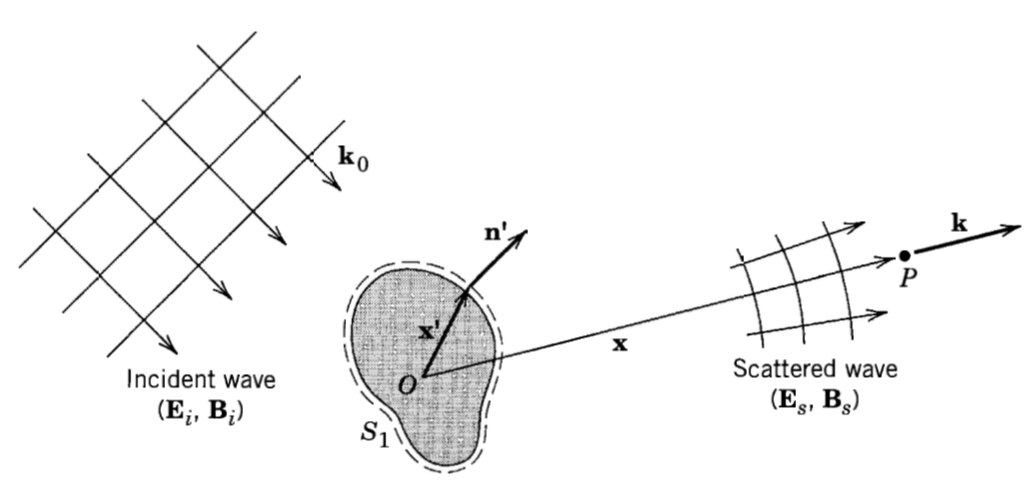
\includegraphics[width=\linewidth]{Immagini/irraggiamento.png}
    		\caption{Onda incidente e onda rifratta}
    		\label{fig:irr}
		\end{figure}
		Dove $E_{i}$ e $E_{s}$ indicano i campi elettrici incidenti e irraggiati (figura \ref{fig:irr},\footnote{è scirtto $E_s$ perchè la $s$ sta per scattered (irraggiato in inglese)} stessa cosa vale per il campo magnetico.\newline
		Visto che $\pscal{\langle\vettore S \rangle}{d\vettore{a}}$ è uguale al flusso di potenza che è uguale a quanti fotoni passano attraverso $d\vettore a$ per unità di tempo per quanta energia ha ognuno di loro, scritto in matematichese $\hbar \omega \phi$=$\hbar \omega \pscal{\vettore j}{d\vettore a}$. Quindi
		\begin{equation}
			\pscal{\langle\vettore S \rangle}{d\vettore{a}}=\hbar \omega \pscal{\vettore j}{d\vettore a}
			\rightarrow
			\langle\vettore S\rangle= \hbar \omega\vettore j
		\end{equation}
		dove $\vettore S=\frac{1}{\mu_0}\Re(\vettore E) \times \Re(\vettore B)$, e $\vettore j$ è lo stesso che va a finire nel denominatore dell'equazione \ref{eq:sez_diff}.\newline
		Ricordiamo la definizione della sezione d'urto differenziale: $\frac{d\sigma}{d\Omega}=N(\Omega)/|j|$ (eq \ref{eq:sez_diff}).
		\[
			\frac{d\sigma}{d\Omega}=\frac{N(\Omega)}{|j|}\cdot\frac{\hbar\omega}{\hbar \omega}=\frac{\hbar \omega N(\Omega)}{|\langle \vettore S_i\rangle|}
		\]
		Adesso concentriamoci col significato di $\hbar \omega N(\Omega)$, esso è uguale a quanti atomi vanno nella direzione dell'angolo $\Omega$ moltiplicato per la loro energia, quindi possiamo dire che se lo moltiplichiamo per la superfice che essi attraversano ($R^2d\Omega $) otteniamo la densità di potenza irraggiata nell'angolo $\omega $, che è uguale a $R^2|\langle \vettore {S}_s \rangle |d\Omega $, quindi mettendo tutto dentro
		\begin{equation}
			\frac{d\sigma}{d\Omega}=\frac{R^2|\langle \vettore S_s(\Omega) \rangle |}{|\langle \vettore S_i\rangle|}
		\end{equation}








\end{document}